\section{Model} 
  \label{model}

  \subsection{ACCESS}  
    \textbf{TODO: Blurb about ACCESS}
    
    \paragraph{Model output} are 4-dimensional: latitude, longitude, vertical level ($\theta$ or $\rho$), and time. Most fields are defined at their grid-box midpoints. Wind speed and direction is defined at the direction-dependent gridbox edge.
    
    
  \subsection{Coupled Fire Model}
    \textbf{TODO: Details about fire model}
    
    \paragraph{Model output} has the same latitude and longitude as ACCESS output, with more frequent time steps and no vertical component.
    A fire front field is produced that is negative where the fire has burnt, and positive elsewhere.
    
  
  
  
  \subsection{Model runs}
    \label{model:runs}
    Over the course of the project the ACCESS-Fire model has been run and updated multiple times, over two regions where large scale forest fires occurred.
    The model runs in a nested fashion, with three to four nests so that the highest resolution possible is produced in a reasonable manner at the site of the fires (e.g. Figure \ref{fig:model:nests}).
    
    The first fire under examination occurred a few kilometers East from Waroona, a suburb South of Perth.
    The second occurred a few hundred kilometres North of Sydney. 
    Both locations are modelled at high resolution using ACCESS-Fire in a nested setup (Figure \ref{fig:model:nests}).
    
    \begin{figure}
      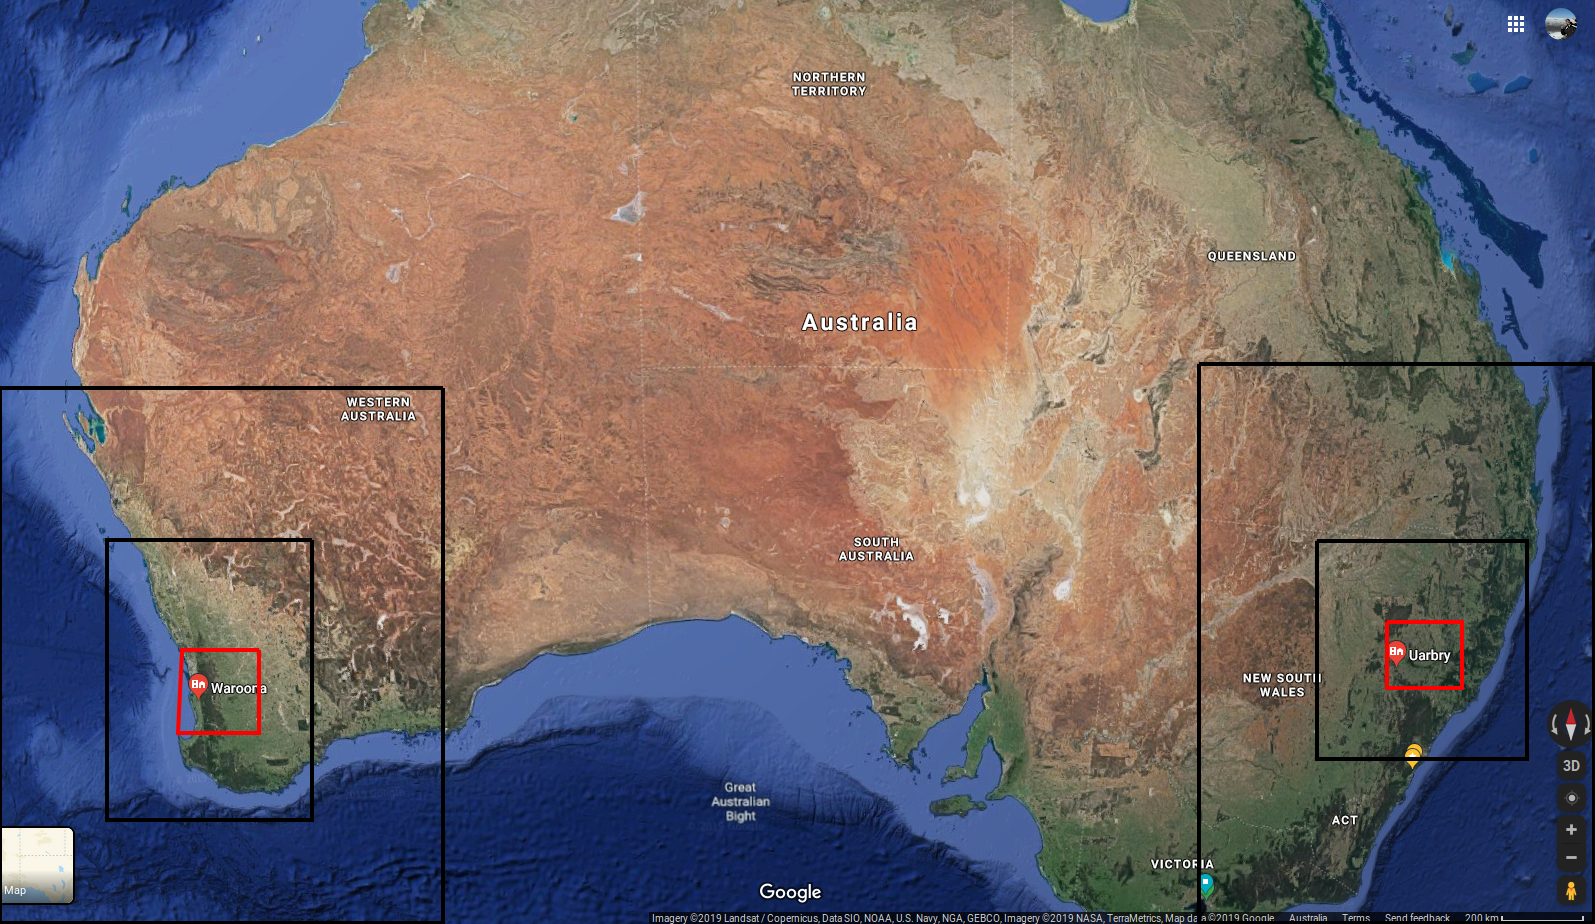
\includegraphics[width=\linewidth]{../../figures/project/Waroona_Uarbry.png}
      \caption{Three nests run by ACCESS-Fire model are shown as black\/red rectangles. 
      The outermost nest has resolution of approximately 3.5 km by 3.5 km, 
      The intermediary Nest is at 1.0 km by 1.0 km, and the smallest nest (red) is at 0.3 km by 0.3 km.
      A fourth nest is sometimes added 
      %taking up the same space as Nest 3 but 
      with .1 km by .1 km resolution.
      Fire coupling is enabled only within the higher resolution (red) nests.}
      \label{fig:model:nests}
    \end{figure}
    
    This report analyses output from the latest iteration of ACCESS-Fire, earlier iterations are listed here as they may help elucidate model parameterisation decisions. 
    \begin{description}
      \item [Waroona\_oldold]
      \begin{itemize}
        \item [] % empty item allows linebreak...
        \item Run in the depths of the past (Oct 2016?)
        \item Output at 30 minute resolution
        \item Meteorology not affected by fire model
        \item slightly different grid to other model runs
      \end{itemize}
      \item [Waroona\_old]
      
      \begin{itemize}
        \item []
        \item Run in Aug, 2018
        \item Output at 30 minute resolution
        \item Run crashed after 21 hours due to runaway model physics (vertical wind speeds > 1km/s)
        \item Fast fire spread parameters
        \item Clear PCB creation around 1100
      \end{itemize}
      
      \item [Waroona\_run1]
      \begin{itemize}
        \item []
        \item Run in Aug, 2019
        \item Output at 10 minute resolution
        \item Increased boundary layer stability to prevent crash
        \item Slower updated fire spread parameters
        \item No real PCB creation seen
      \end{itemize}
      
      \item [Waroona\_run2]
      \begin{itemize}
        \item []
        \item Run in Dec, 2019 (Raijin's last encore)
        \item Output at 10 minute resolution
        \item Increased boundary layer stability
        \item Fire spread parameters: Faster (older, matching Waroona\_old)
        \item can be compared to Waroona\_run2uc, which has identical settings but no fire coupling
      \end{itemize}
      
      \item [Waroona\_run3]
      \begin{itemize}
        \item []
        \item Run in Feb, 2020 (GADI)
        \item Output at 10 minute resolution
        \item Increased boundary layer stability
        \item Fire spread parameters: ?
      \end{itemize}
    \end{description}
    
    \begin{figure}
      \includegraphics[width=\linewidth]{../../figures/project/fireplan/waroona_firespread.png}
      \caption{Model run fire fronts at start of burn and end of simulation}
      \label{fig:model:firespread_waroona}
    \end{figure}
    
    
  \subsection{Modelled Weather}
    \label{model:weather_summary}
    
    Weather is examined at various scales by sub-selecting extents and vertical levels, then viewing horizontal and vertical winds, cloud content, and other available metrics. This section outlines in chronological order the overall weather in the latest model run for each site.
    
    \paragraph{The Waroona} simulation starts 1 hour before midnight, Figure \ref{fig:model:waroona_summary_timeseries} shows the near-fire surface weather metrics over the first 24 hours.
    Winds from ESE near the surface form horizontal rolls for several hours (Figure TODO). Fire ignition occurs after about 5 hours (4AM), and progresses westwards in the easterly winds. 
    The fire is seen to influence vertical motion a long way down-wind, before clear East-West oriented horizontal rolls occur in the vertical motion around midday. 
    At about 2 in the afternoon, some westward winds occur at the base of the escarpment, causing updraughts and disrupting the horizontal rolls.
    Coincidentally the vertical motion near the fire front can be seen to have pushed into the upper troposphere leading to heightened cloud activity (Figure \ref{fig:model:weather_summary_updraught}), This feature is discussed more in Section \ref{pcb}.
    Easterly winds re-establish dominance by 7PM, getting stronger especially down the escarpment until the end of the simulation.
    The fire spreads down the escarpment on this first evening exactly when these winds pick up, this feature is discussed in more detail in Section \ref{emberstorm}.
    % Initial weather, horizontal rolls, ignition, spread and PCB, evening downslope run.
    
    \begin{figure}
      \includegraphics[width=\linewidth]{../../figures/waroona_run3/weather_summary/timeseries.png}
      \caption{%
        Top panel shows a top down satellite view near Waroona, with the fire outline after 24 hours shown in red. A blue rectangle shows the area that is averaged at each time step shown in the bottom two panels.
        The second panel shows several parameters over time, on 3 different y-axes, firepower and PFT share the left y-axis, cloud cover fraction and RH share the right-most y-axis.
        "Cloud cover" marks the fraction of the blue rectangle (top panel) where more than 0.1 g\/kg ice and water content in air occurs. 
        The blue circles are filled when the heaviest 25\% of total cloud content occurs, and half filled for the second highest 25\%.
        The third panel shows surface mean wind speed and direction, including grey shading within the inter-quartile range and a triangle shows the maximum wind speed.
        }
      \label{fig:model:waroona_summary_timeseries}
    \end{figure}
    
    \begin{figure}
      \includegraphics[width=\linewidth]{../../figures/waroona_run3/weather_summary/fig_201601060600.png}
      \caption{Left panels show horizontal wind speed (coloured contour map) and wind direction (arrows).
      Right panels show vertical wind speed (coloured contour map) and cloud content (diagonal stippling).
      The wind speeds are averaged into vertical bins based on height above the ground, showing lower to higher altitudes from the first row to the last row respectively.
      Cloud content is summed within each vertical bin, and the areas marked have at least 0.1 gkg$^{-1}$ of water and ice.}
      \label{fig:model:weather_summary_updraught}
    \end{figure}
    
    \paragraph{The Sir Ivan} simulation starts at 7AM under north westerly winds, Figure \ref{fig:model:sirivan_summary_timeseries} outlines the surface weather over 24 hours.
    Fire ignition occurs after 3.5 hours, initially spreading east before the wind swings around to push the fire towards the north along a long east to west fire front after about 3 hours. 
    Northward fire spread continues for the rest of the simulation, with a marked storm cloud produced at approximately 5PM.
    
    \begin{figure}
      \includegraphics[width=\linewidth]{../../figures/sirivan_run1/weather_summary/timeseries}
      \caption{%
        Top panel shows a top down satellite view near Sir Ivan, with the fire outline after 24 hours shown in red. A blue rectangle shows the area that is averaged at each time step shown in the bottom two panels.
        The second panel shows several parameters over time, on 3 different y-axes, firepower and PFT share the left y-axis, cloud cover fraction and RH share the right-most y-axis.
        "Cloud cover" marks the fraction of the blue rectangle (top panel) where more than 0.1 g\/kg ice and water content in air occurs. 
        The blue circles are filled when the heaviest 25\% of total cloud content occurs, and half filled for the second highest 25\%.
        The third panel shows surface mean wind speed and direction, including grey shading within the inter-quartile range and a triangle shows the maximum wind speed.}
      \label{fig:model:sirivan_summary_timeseries}
    \end{figure}
  
  \subsection{Data flow}
    \textbf{TODO: Data flow diagram for project}
